\chapter{System Sequenz Diagramm und Operation Contracts}

\section{System Sequence Diagram, SSD}
Use Cases beschreiben wie Externe Aktoren mit dem System interagieren.
SSD beschreiben einzelne System Operationen

\begin{figure}[!h]
    \centering
    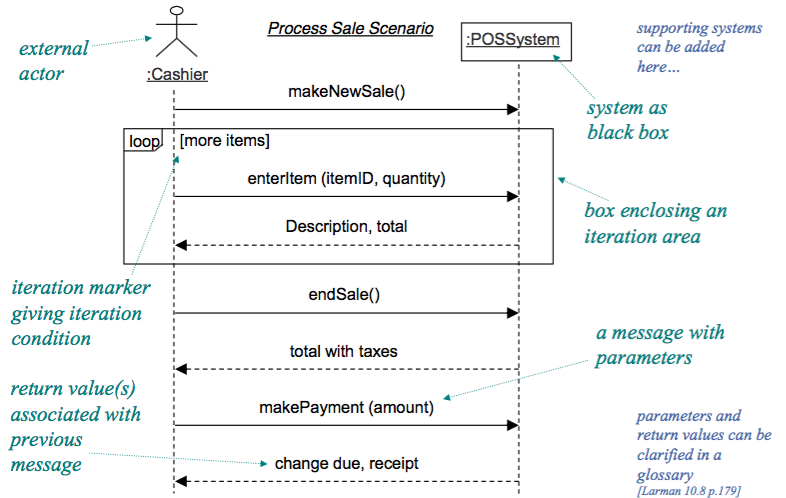
\includegraphics[scale=0.5]{ssd}
    \caption{System Sequence Diagram}
\end{figure}

\section{Operation Contracts}
Contracts werden in einer Deklarativen Art und Weise geschrieben. Fokus auf
was getan werden muss und nicht wie. Hilfreich für System Design, die sich um
das ,,wie'' beschäftigen müssen. \\
Sobald System Operationen identifiziert werden, beschreiben Operation Contracts
diese mehr im Detail.

\subsection{Operaton Contract Schema}
Werden oft verwendet, wenn Komlpexität vorherrscht. Nicht zwingend notwendig,
wenn in eindeutigem Kontext.
\begin{compactitem}
    \item \textbf{Operation}: Name der Operation und Parameter
    \item \textbf{Cross References}: (optionale) Use Cases, in denen diese Operation
    verwendet wird.
    \item \textbf{Preconditions}: Zustand, der vor Ausführung der Operation herrscht.
    \item \textbf{Postconditions}: Zustand des Domain Models nach Beendigung der
    Operation.
\end{compactitem}
